\documentclass[13pt,aspectratio=169]{beamer}

\usetheme{Rochester}
\usecolortheme{default}

\usefonttheme[onlymath]{serif}
\usepackage[numbers, sort&compress]{natbib}
\bibliographystyle{abbrvnat}

\usepackage{subfigure}
\usepackage{amsmath,amssymb,amsfonts}
\usepackage{algorithm, algorithmic}
\usepackage{booktabs}
\usepackage{url}

\usepackage{tikz}
\usetikzlibrary{bayesnet, plotmarks, calc, arrows, shapes, positioning, automata}

\usepackage{pgfplots}
\usepgfplotslibrary{groupplots, statistics}
\pgfplotsset{
    compat=1.15,
    only if/.style args={entry of #1 is #2}{
        /pgfplots/boxplot/data filter/.code={
            \edef\tempa{\thisrow{#1}}
            \edef\tempb{#2}
            \ifx\tempa\tempb
            \else
                \def\pgfmathresult{}
            \fi
        }
    }
}

% Parameters
\newcommand{\tbuf}{\beta}
\newcommand{\trate}{\alpha}
\newcommand{\scoeff}{\gamma}
\newcommand{\lookback}{L}
\newcommand{\nactors}{K}
\newcommand{\timeout}{T}
% Variables
\newcommand{\vsym}{r}
\newcommand{\tsym}{t}
\newcommand{\msym}{m}
\newcommand{\graph}{G}
\newcommand{\iactor}{k}
% Operators
\DeclareMathOperator{\argmax}{\arg\max}
\DeclareMathOperator{\nhood}{ne}
\DeclareMathOperator{\mrr}{mrr}
\newcommand{\init}{\msym_0}
\newcommand{\curr}{\vsym}
\newcommand{\ival}{\vsym_0}
\newcommand{\itime}{\tsym_0}
\newcommand{\msg}[2]{\msym_{#1 \rightarrow #2}}
\newcommand{\mval}[2]{\vsym_{#1 \rightarrow #2}}
\newcommand{\mtime}[2]{\tsym_{#1 \rightarrow #2}}
\newcommand{\reach}{\msym}
\newcommand{\estreach}{\hat{\msym}}
\newcommand{\card}[1]{\left\vert #1 \right\vert}
\newcommand{\vpath}[2]{#1 \rightarrow #2}
% Sets
\newcommand{\contacts}{\mathcal{C}}
\newcommand{\rscores}{\mathcal{R}}
\newcommand{\scores}{\mathcal{S}}
\newcommand{\edges}{\mathcal{E}}
\newcommand{\variables}{\mathcal{V}}
\newcommand{\factors}{\mathcal{F}}
\newcommand{\actors}{\mathcal{G}}
\newcommand{\pathsym}{\mathcal{P}}

\title[ShareTrace]{ShareTrace: Contact Tracing with the Actor Model}

\author[Tatton et al.]{Ryan Tatton\inst{1} \and Erman Ayday\inst{1} \and Youngjin Yoo\inst{2} \and Anisa Halimi\inst{3}}

\institute[CWRU]
{
  \inst{1}%
  Department of Computer and Data Sciences\\
  Case Western Reserve University
  \and
  \inst{2}
  Deparment of Design and Innovation\\
  Case Western Reserve University
  \and
  \inst{3}
  IBM Research Europe
}

\date{IEEE HealthCom, October 2022}
\setbeamertemplate{navigation symbols}{}

\begin{document}

\begin{frame}
	\maketitle
\end{frame}

\begin{frame}{Motivation}
\begin{itemize}
	\item Proximity-based contact tracing relies on mobile-device interaction to estimate infection spread \cite{Ahmed2020, Martin2020, Wen2020, Raskar2020, Cho2020, Dar2020, Lucivero2020, Kuhn2021}
	\item ShareTrace is a privacy-preserving, proximity-based approach that estimates a user's infection risk based on their symptoms, direct contacts, \emph{and} indirect contacts
	\item Previous work \cite{Ayday2021} evaluted efficacy, but not scalability or efficiency
\end{itemize}
\end{frame}

\begin{frame}{Definitions}
\begin{itemize}
\item \emph{Risk score} $(\vsym, \tsym)$: a timestamped probability where $\vsym \in [0, 1]$ and $\tsym \geq 0$
	\begin{itemize}
	\item \emph{Symptom score}: prior infection probability; only considers user symptoms \cite{Menni2020}
	\item \emph{Exposure score}: posterior infection probability; accounts for (in)direct contact
	\end{itemize}
\item \emph{Factor graph} $\graph = (\variables, \factors, \edges)$: a bipartite graph \cite{Kschischang2001}
	\begin{itemize}
	\item $\variables$: variable vertices, where a variable vertex $v \in \variables$ represents a user
	\item $\factors$: factor vertices, where a factor vertex $f(u, v) \in \factors$ represents a contact
	\item $\edges$: edges incident between the sets $\variables$ and $\factors$
	\end{itemize}
\item \emph{Message} $\msg{u}{v} = \{(\vsym, \tsym),\ldots\}$: a set of risk scores sent from vertex $u$ to vertex $v$
\end{itemize}
\end{frame}

\begin{frame}{Proposed Scheme}
\begin{figure}
\centering
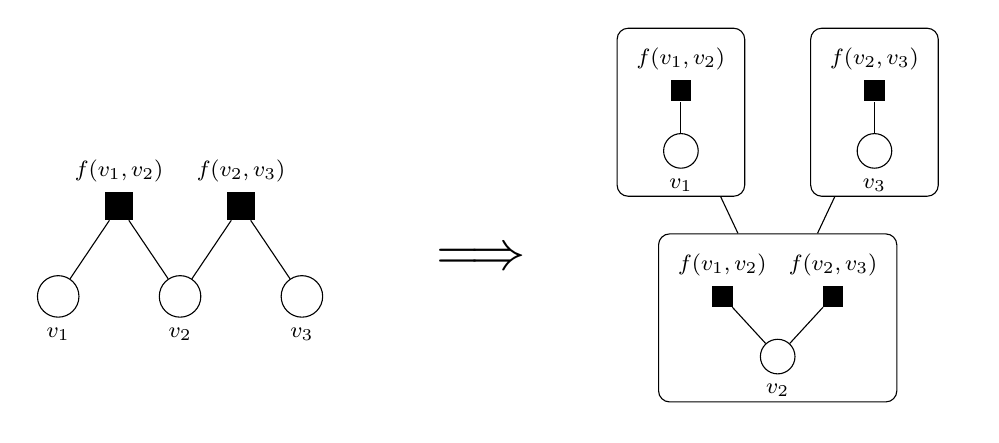
\begin{tikzpicture}[baseline={(0,0)}, ampersand replacement=\&]
\matrix[row sep=2em, column sep=-0.5em] at  (-5, 0.25)
{%
	\& \factor[minimum size=1em] {f12} {above:$f(v_1, v_2)$} {} {}; \&\&
	\factor[minimum size=1em] {f23} {above:$f(v_2, v_3)$} {} {}; \& \\
	\node[latent, label=below:$v_1$, minimum size=1.5em] (v1) {}; \&\&
	\node[latent, label=below:$v_2$, minimum size=1.5em] (v2) {}; \&\&
	\node[latent, label=below:$v_3$, minimum size=1.5em] (v3) {}; \\
};
\edge[-] {v1} {f12};
\edge[-] {v2} {f12};
\edge[-] {v2} {f23};
\edge[-] {v3} {f23};
\hspace{-5.5em}\scalebox{2}{$\implies$}
\matrix[row sep=5em, column sep=2em] at (3, 0)
{%
	\node[latent, label=below:$v_1$, minimum size=1.25em] (v1) {}; \&
	\& \node[latent, label=below:$v_3$, minimum size=1.25em] (v3) {}; \\
	\& \node[latent, label=below:$v_2$, minimum size=1.25em] (v2) {}; \& \\
};
\factor[minimum size=0.75em, above= of v1] {f121} {above:$f(v_1, v_2)$} {} {};
\factor[minimum size=0.75em, above= of v2, xshift=-2em] {f122} {above:$f(v_1, v_2)$} {} {};
\factor[minimum size=0.75em, above= of v2, xshift=2em] {f232} {above:$f(v_2, v_3)$} {} {};
\factor[minimum size=0.75em, above= of v3] {f233} {above:$f(v_2, v_3)$} {} {};

\plate{p1} {(v1)(f121)(f121-caption)} {};
\plate{p2} {(v2)(f122)(f232)(f122-caption)(f232-caption)} {};
\plate{p3} {(v3)(f233)(f233-caption)} {};

\edge[-] {v1} {f121};
\edge[-] {v2} {f122};
\edge[-] {v2} {f232};
\edge[-] {v3} {f233};
\edge[-] {p1} {p2};
\edge[-] {p2} {p3};
\end{tikzpicture}
\caption{Apply one-mode projection on the factor graph (left) to get the contact network (right)}
\label{fig:contact-network}
\end{figure}
\end{frame}

\begin{frame}{Proposed Scheme}
\begin{itemize}
	\item Reformulate the factor graph as a \emph{temporal contact network} \cite{Holme2012, Holme2015}:
		\begin{equation*}
				\contacts = \{(u, v, t) \mid u, v \in \variables; u \neq v; \tsym \geq 0\}
		\end{equation*}
	\item Partition the contact network into $K$ subnetwork \emph{actors} $\graph_k \in \graph$ \cite{Agha1986, Baker1977}
	\item Send each actor its initial risk scores (i.e., previous exposure and symptom scores)
	\item Actors non-iteratively pass messages (\emph{risk scores}) until convergence
	\item Assumption: risk transmission is incomplete; use a \emph{transmission rate} of $\trate = 0.8 \in (0, 1)$ \cite{Hamner2020}
\end{itemize}
\end{frame}

\begin{frame}{Proposed Scheme}
\begin{itemize}
\item Only propagate messages if they are likely to change the risk score of other users in the network
\item \emph{Send coefficient} $\scoeff$ parametrizes the trade-off between accuracy and efficiency of non-iterative message passing
\item A vertex $u$ only sends a message $\msg{u}{v}$ if
	\begin{itemize}
	\item it is close in value to its initial message: $\mval{u}{v} \geq \scoeff \cdot \ival(u)$; and
	\item it is at least as old as its initial message: $\mtime{u}{v} \leq \itime(u)$
	\end{itemize}
\item Ensures convergence when $\trate < 1$ and $\scoeff > 0$
\end{itemize}
\end{frame}

\begin{frame}{Message Reachability}
\begin{itemize}
\item In temporal network theory, a \emph{time-respecting path} (TRP) is a sequence of nondecreasing contacts.
	\begin{itemize}
	\item Vertex $v$ is \emph{temporally reachable} from vertex $u$ if there exists a TRP from $u$ to $v$
	\end{itemize}
\item Message-passing on a temporal network may not require temporal reachability
\item \emph{Message reachability} from vertex $u$ to vertex $v$ is the number of edges along the shortest path $\pathsym = \vpath{u}{v}$ that satisfy the message-passing constraints,
	\begin{equation*}
		\reach(u, v) = \sum_{(i, j) \in \pathsym} f(u, i, j, v),
	\end{equation*}
where $f(u, i, j, v) = 1$ if all constraints are satisfied and $f(u, i, j, v) = 0$ otherwise
\end{itemize}
\end{frame}

\begin{frame}{Message Reachability: Risk Propagation}
Let $H(x) = \mathbf{1}_{x \geq 0}$ be the \emph{Heaviside step function}. Then
\begin{equation*}
    \reach(u) = \underset{\pathsym}{\max} \left\{\sum_{(i, j) \in \pathsym} f_c(u, i, j) \cdot f_{\vsym}(u, i) \cdot f_{\tsym}(u, i) \right\}
\end{equation*}
where users are enumerated $0, 1, \ldots, \card{\pathsym} - 1$, ; and
	\begin{itemize}
	\item Contact-time constraint: $f_c(u, i, j) = H(\tsym_{ij} + \tbuf - \itime(u))$
		\begin{itemize}
		\item \emph{Time buffer} $\tbuf \geq 0$ accounts for incubation and delayed symptom reporting
		\end{itemize}
	\item Risk-score value constraint: $f_r(u, i) = H(\trate^i \cdot \ival(u) - \scoeff \cdot \ival(i))$
		\begin{itemize}
		\item Risk score values exponentially decrease as they propagate from their source user
		\end{itemize}
	\item Risk-score time constraint: $f_t(u, i) = H(\itime(i) - \itime(u))$
		\begin{itemize}
		\item Older risk scores are less likely to be propagated
		\end{itemize}
	\end{itemize}
\end{frame}

\begin{frame}{Message Reachability: Risk Propagation}
\begin{itemize}
\item We can estimate $\reach(u)$ by relaxing the temporality constraints:
	\begin{equation*}
	\trate^i \cdot \ival(u) - \scoeff \cdot \ival(i) = 0 \overset{\text{solve for $i$}}{\Longrightarrow} \estreach(u, v) = \log_{\trate}\left\{\scoeff \cdot \frac{\ival(v)}{\ival(u)} \right\}
	\end{equation*}
\item (Estimated) message reachability of a vertex $u \in \variables$:
	\begin{align*}
		\reach(u) = \max \{\reach(u, v) \mid v \in \variables \} \\
		\estreach(u) = \max \{\estreach(u, v) \mid v \in \variables \}
	\end{align*}
\end{itemize}
\end{frame}

\begin{frame}{Message Reachability: Significance}
\begin{itemize}
	\item Generalizes temporal reachability to account for message-passing semantics
	\item Quantifies the communication complexity of a given algorithm
	\item RP: higher message reachability $\implies$ more users at risk
	\item RP: higher send coefficient $\scoeff$ $\implies$ higher communication cost (optimize!)
\end{itemize}
\end{frame}

\begin{frame}{Evaluation}
\begin{itemize}
\item What is the optimal value for the send coefficient?
\item How do the transmission rate and send coefficient affect accuracy and efficiency?
\item How accurate is estimated message reachability?
	$$\text{\emph{Message-reachability ratio}}:~\mrr(u) = \frac{\reach(u)}{\estreach(u)}$$
\item What is the runtime performance of risk propagation?
\item Synthetic graphs:
	\begin{itemize}
	\item Random geometric graphs (RGGs) \cite{Dall2002}
	\item Benchmark graphs (LFRGs) \cite{Lancichinetti2008}
	\item Clustered scale-free graphs (CSFGs) \cite{Holme2002}
	\end{itemize}
\end{itemize}
\end{frame}

\begin{frame}{Evaluation: SocioPatterns Networks}
\begin{figure}
   	\centering
   	\subfigure[High school: 180/2,220 \cite{Fournet2014}]{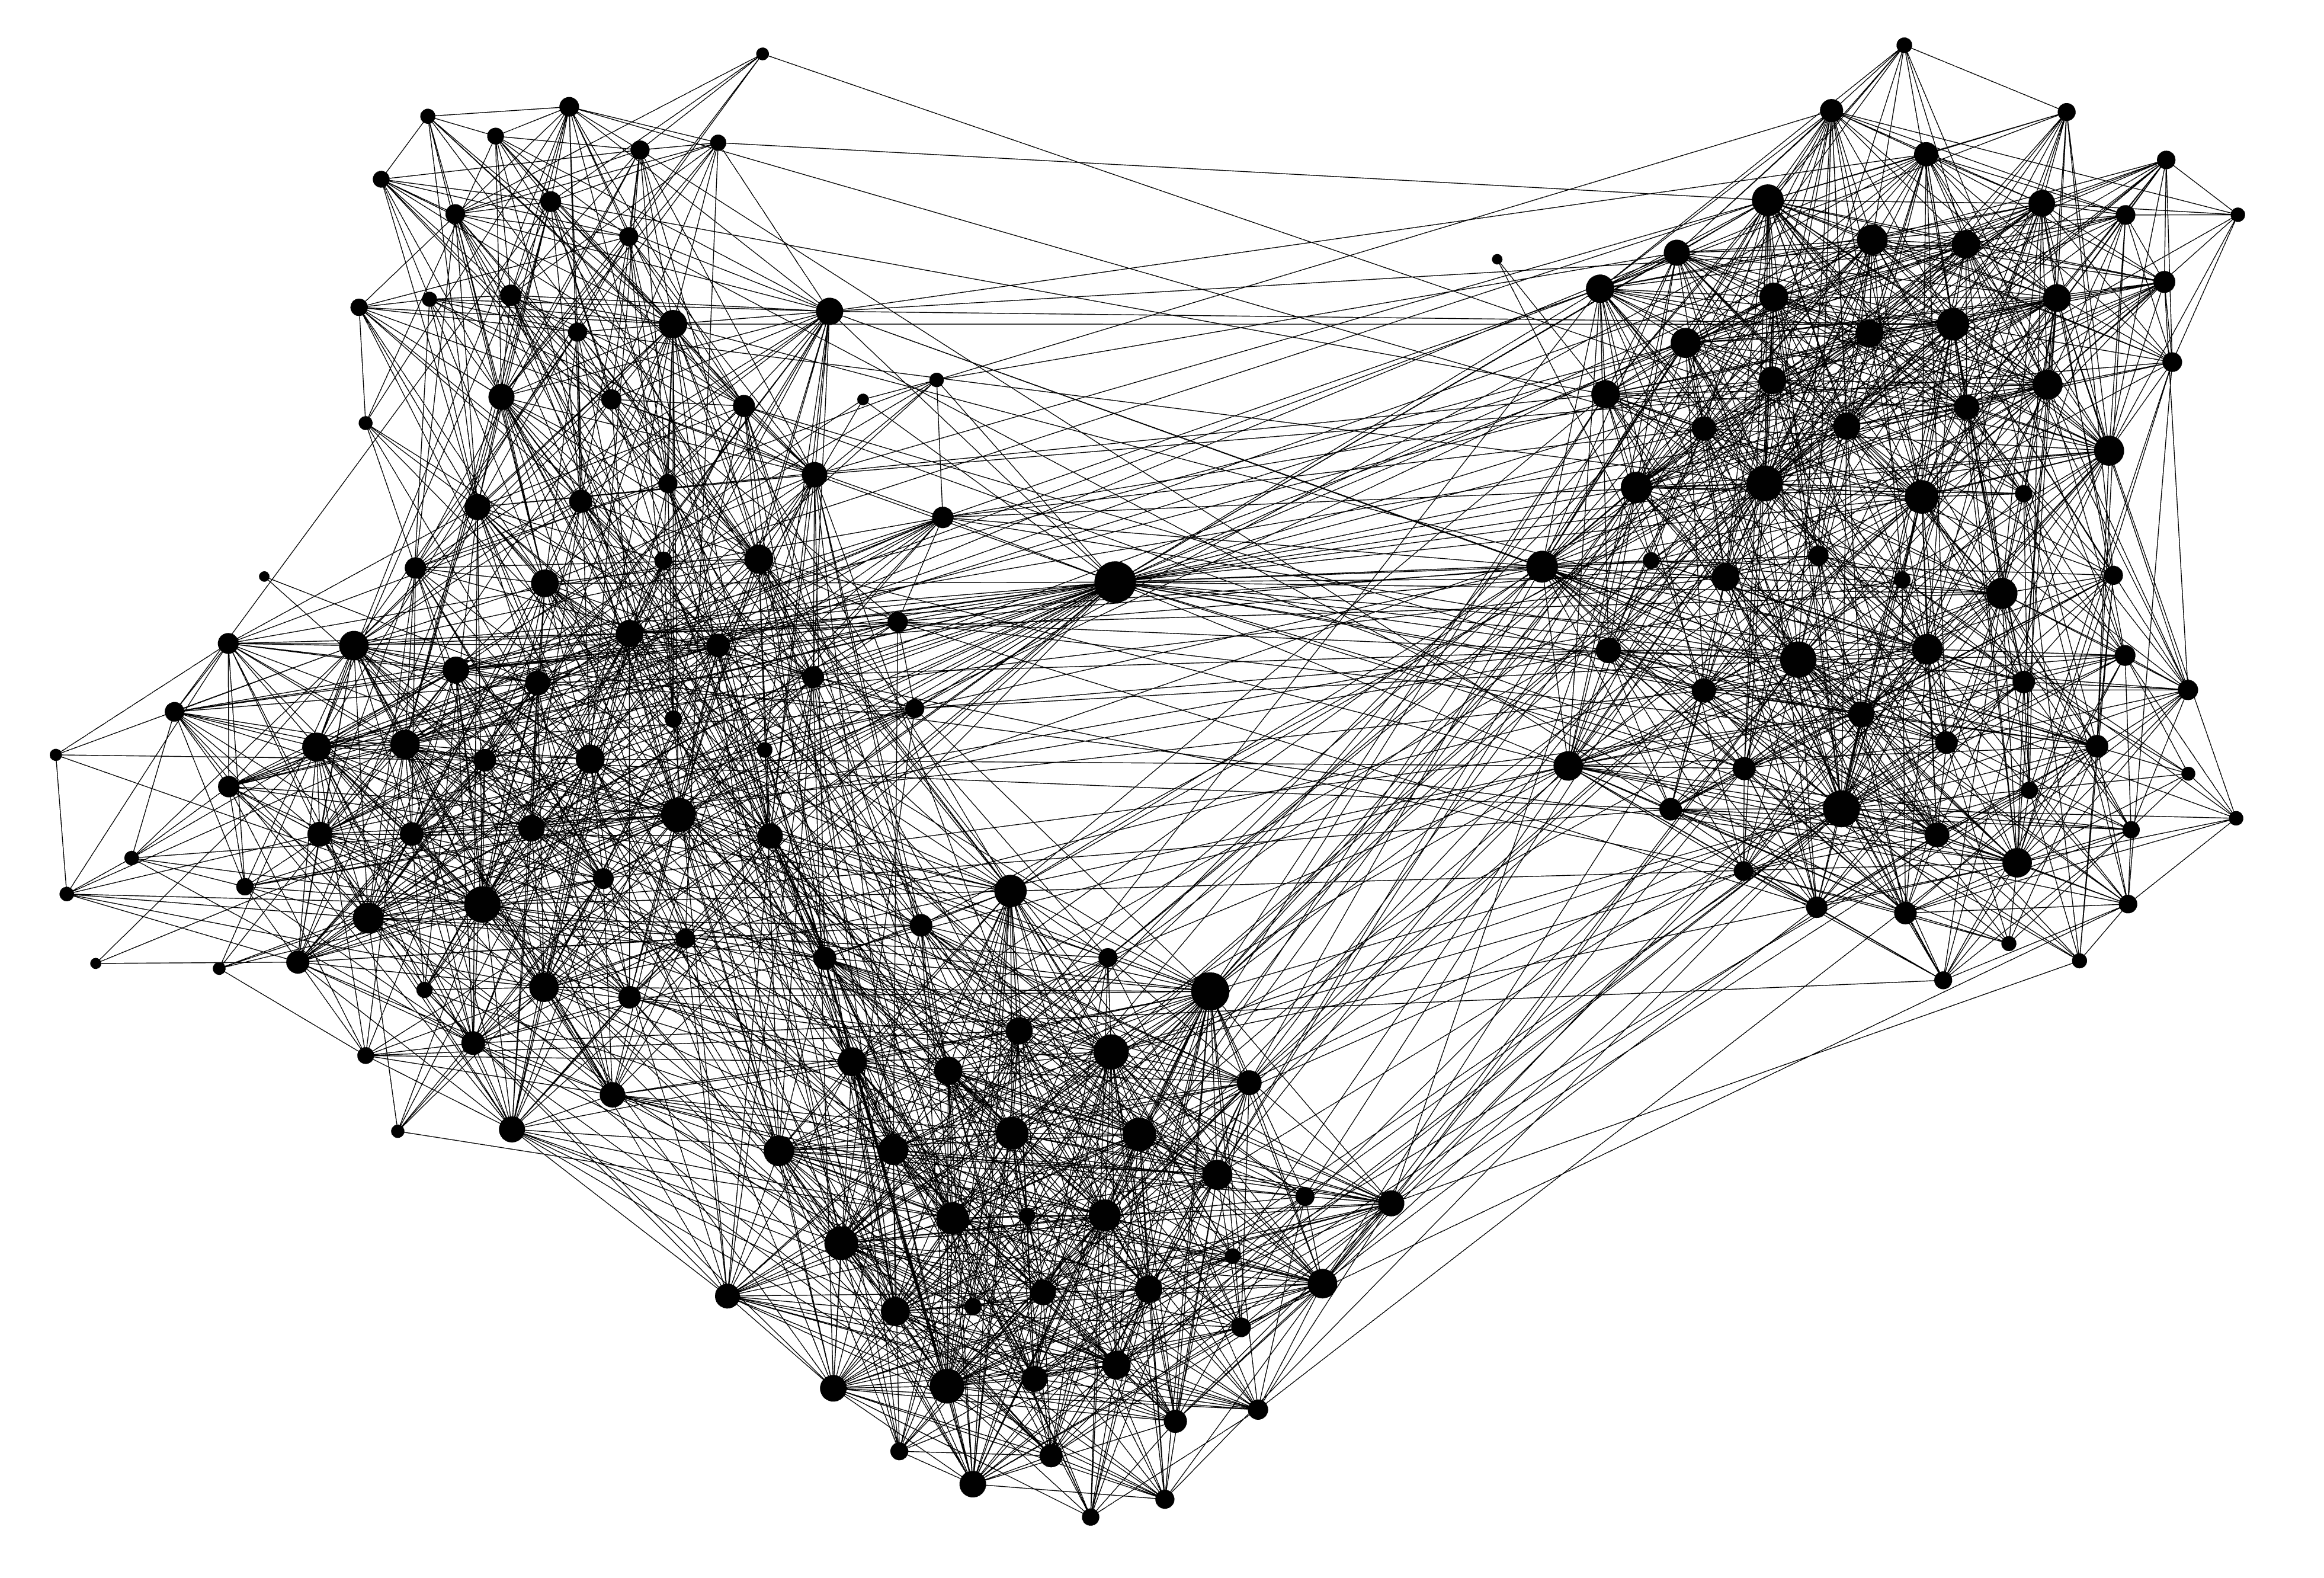
\includegraphics[width=0.32\columnwidth]{anc/highschool12}} \hfill
	\subfigure[Workplace: 217/4,274 \cite{Genois2018}]{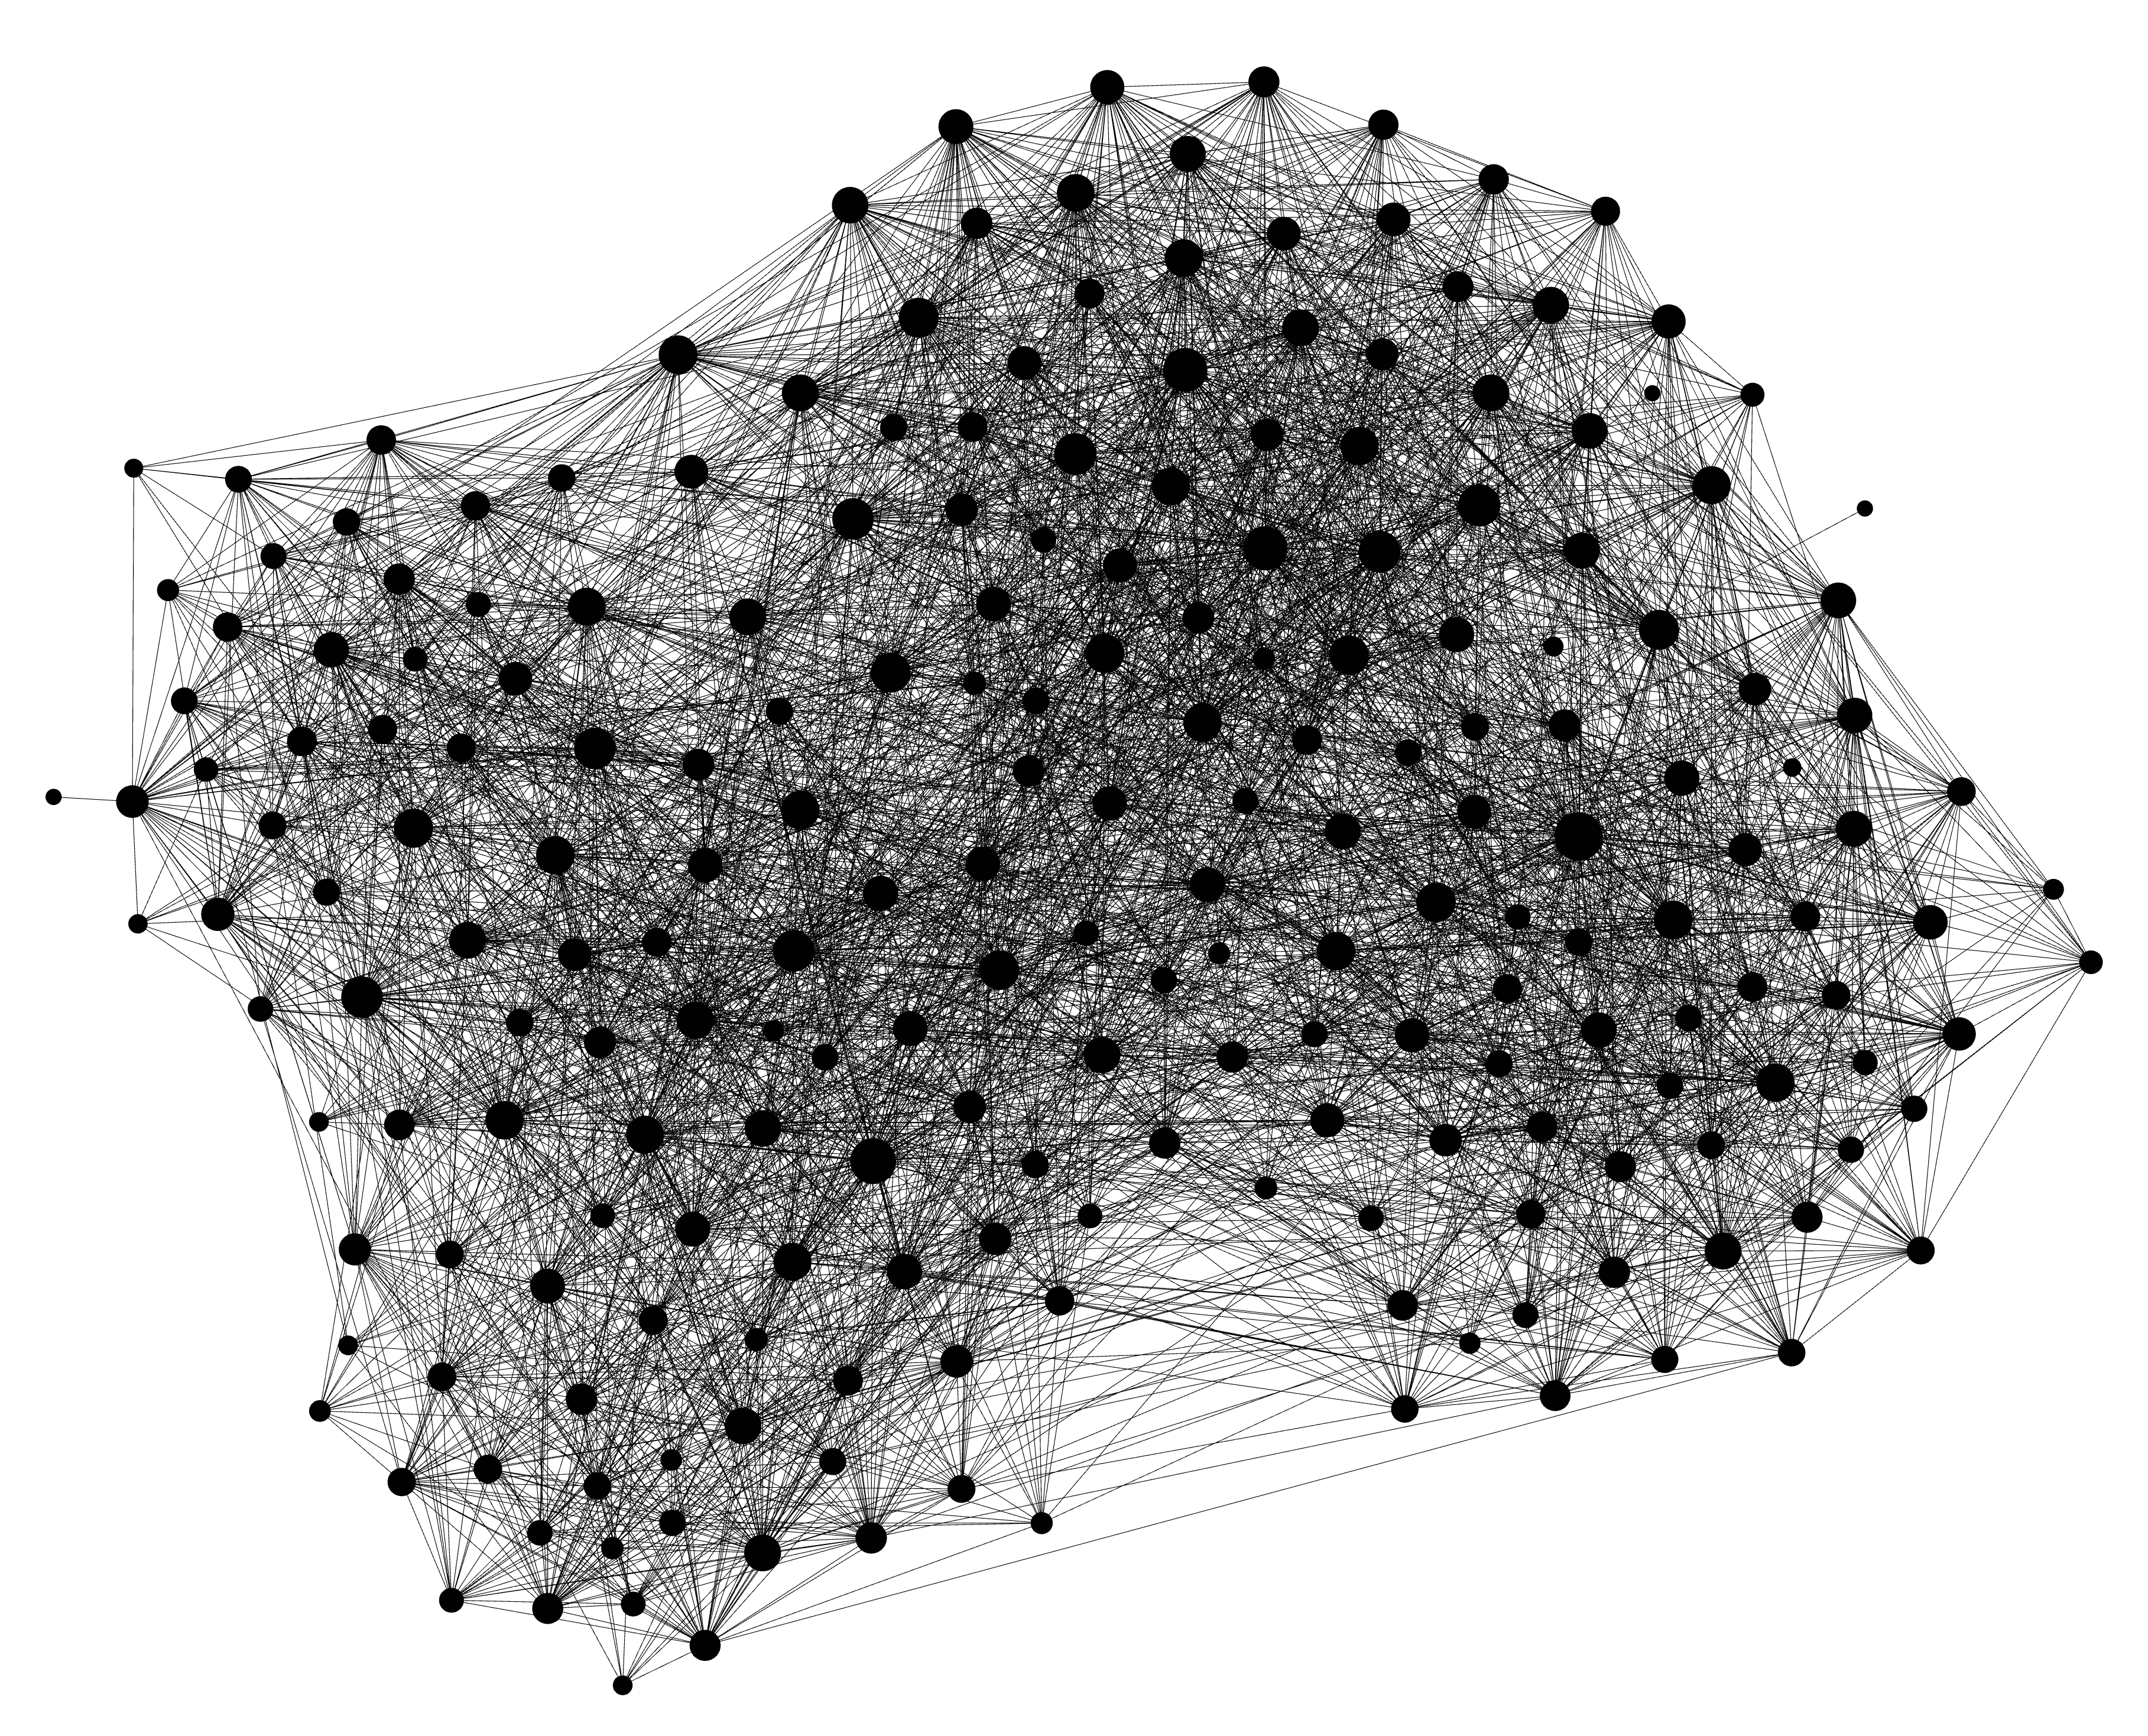
\includegraphics[width=0.32\columnwidth]{anc/workplace}} \hfill
	\subfigure[Conference: 403/9,565 \cite{Genois2018}]{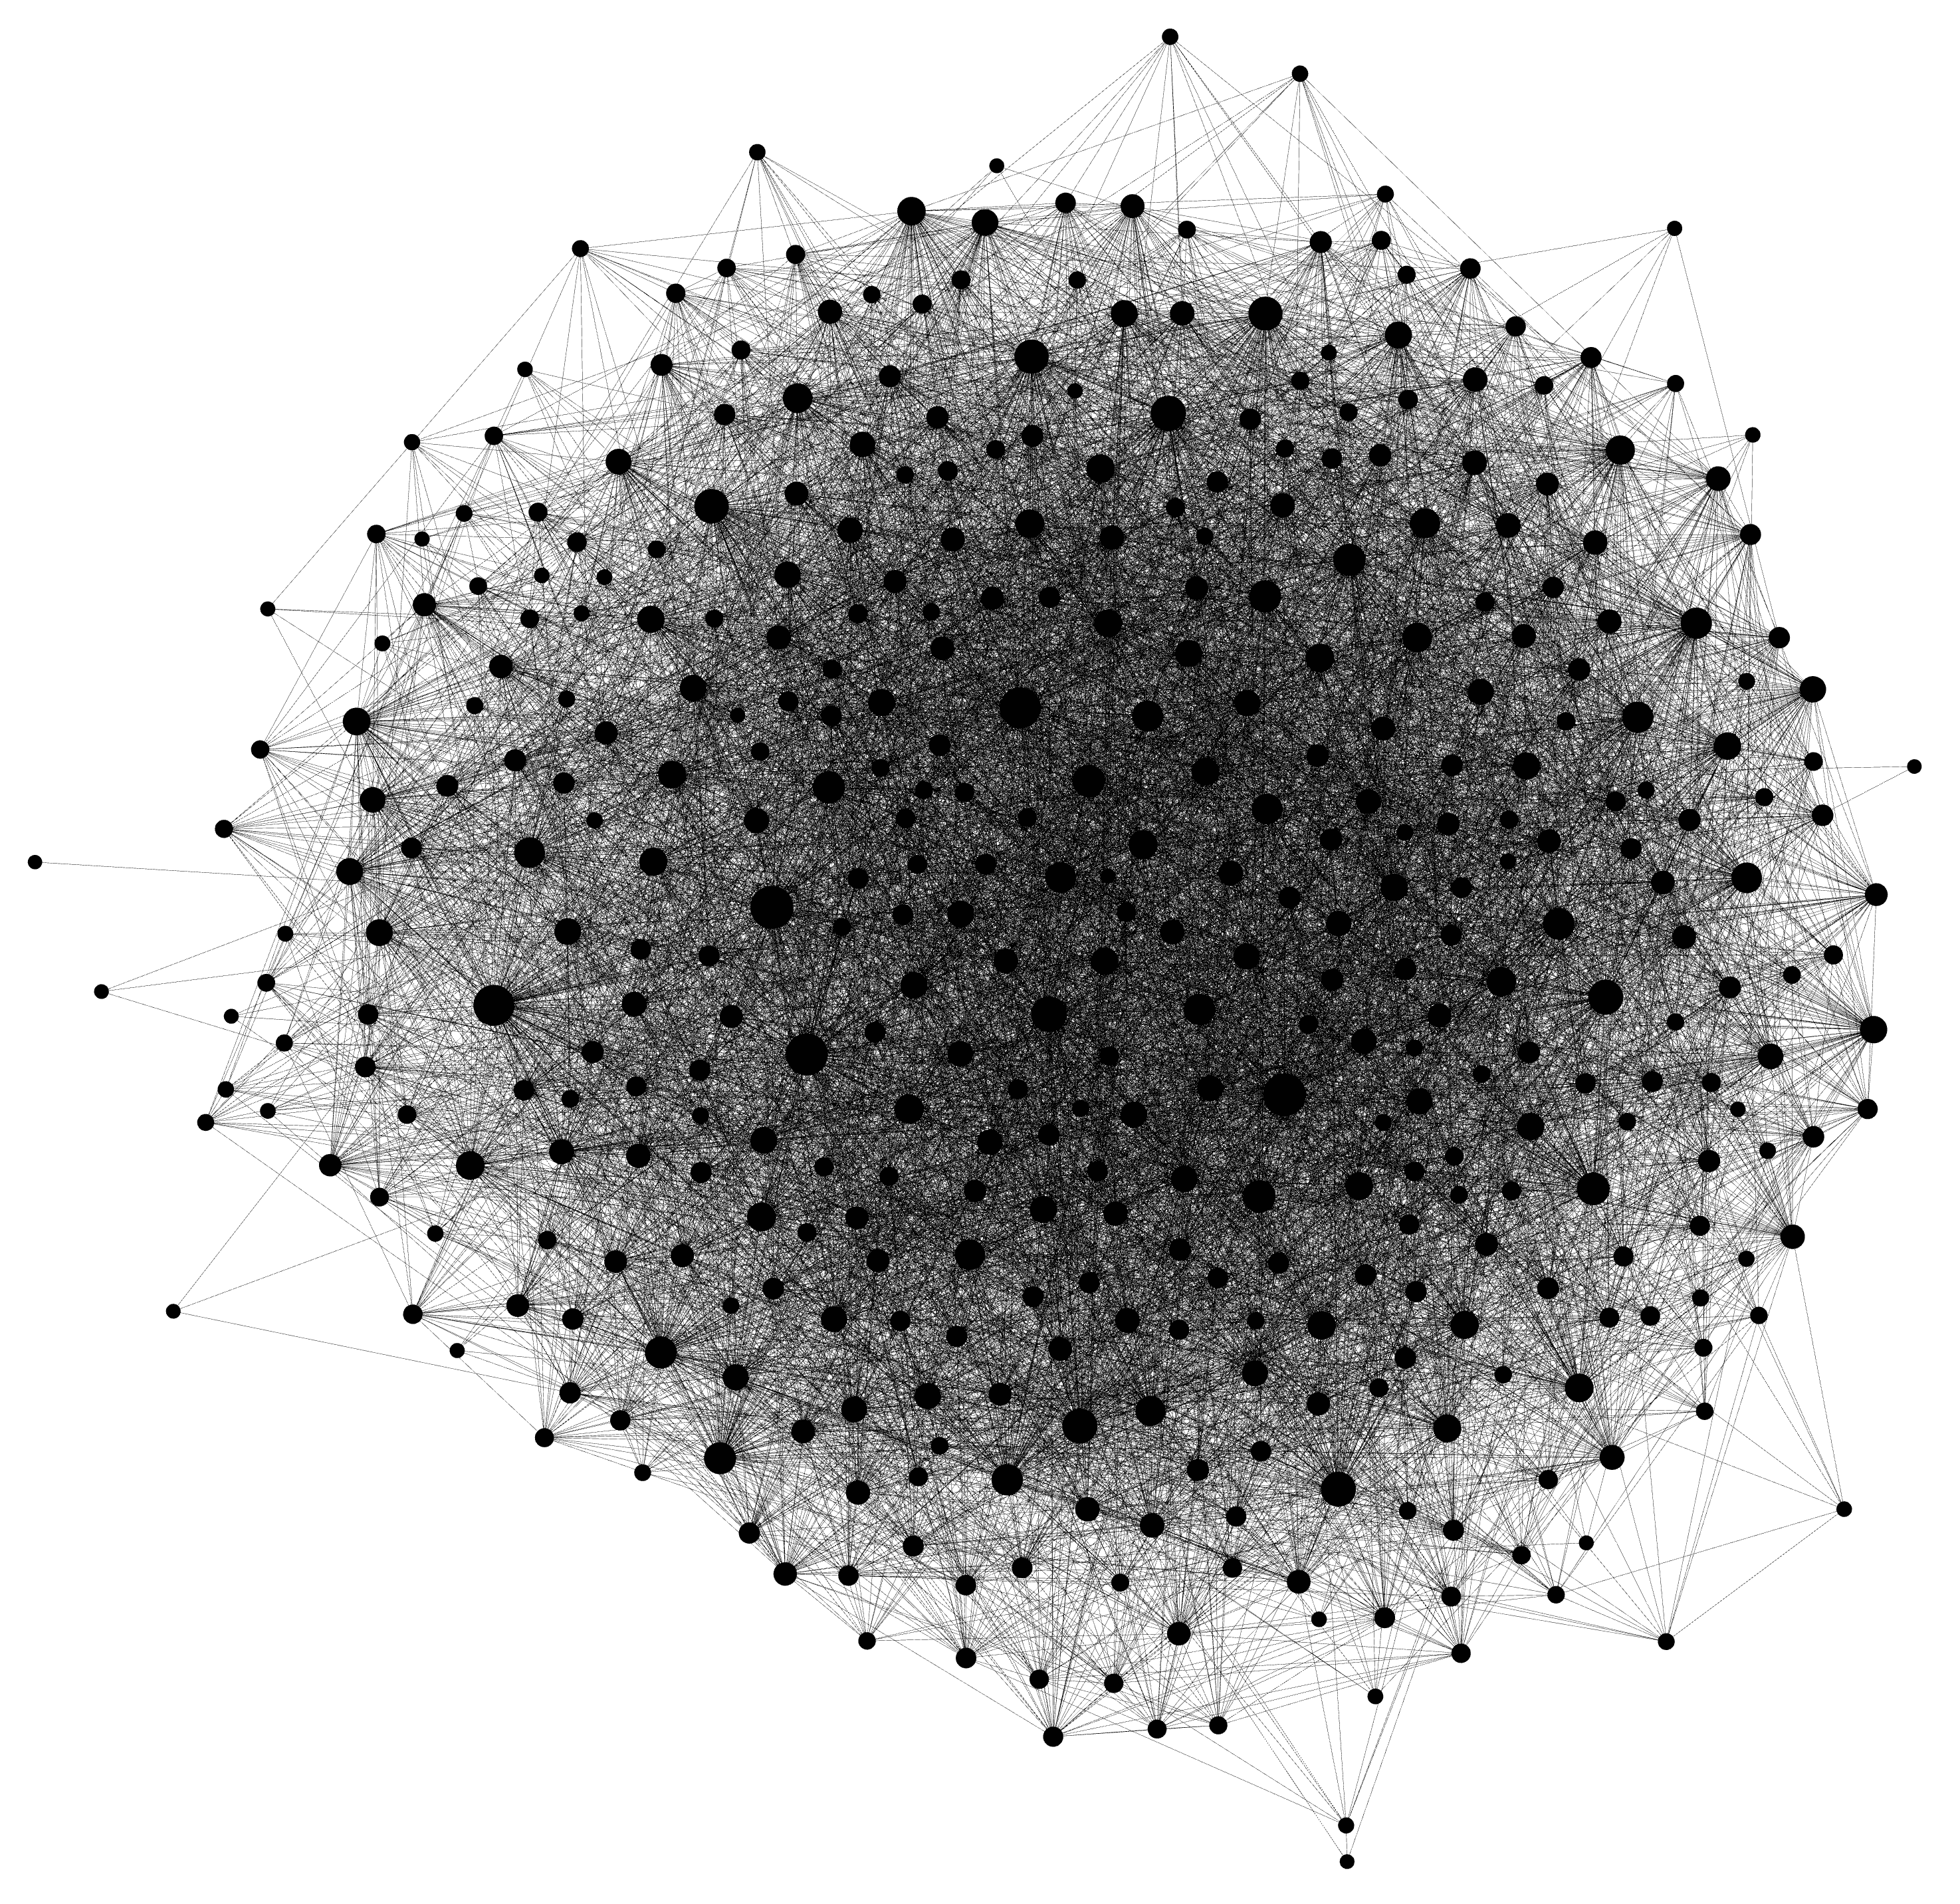
\includegraphics[width=0.32\columnwidth]{anc/conference}}
	\caption{SocioPatterns contact networks (number of users / number of contacts). Edges represents the most recent time of contact (duration $\geq$ 20s).}
\end{figure}
\end{frame}

\begin{frame}{Results: Efficiency}
\begin{figure}
\centering
\begin{tikzpicture}
{\small
\begin{groupplot}[
group style={
	group size=3 by 1,
	xlabels at=edge bottom,
	ylabels at=edge left
},
boxplot,
table/col sep=comma,
boxplot/draw direction=y,
xtick distance=2,
scaled x ticks={base 10:-1},
width=0.35\textwidth,
height=0.29\textwidth,
ymin=-0.1,
ytick distance=0.2,
xtick scale label code/.code={},
xlabel={Send coefficient}
]
\nextgroupplot[table/y=NormalizedUpdates,title={Normalized update count}]
\foreach \t in {1,...,10} {
	\addplot[color=black] table[only if={entry of SendTolerance is \t}]{anc/tolerance-updates.csv};
}%
\nextgroupplot[table/y=NormalizedRuntimeInSeconds,title={Normalized runtime}]
\foreach \t in {1,...,10} {
	\addplot[color=black] table[only if={entry of SendTolerance is \t}]{anc/tolerance-runtime.csv};
}%
\nextgroupplot[table/y=NormalizedMessages,title={Normalized message count}]
\foreach \t in {1,...,10} {
	\addplot[color=black] table[only if={entry of SendTolerance is \t}]{anc/tolerance-messages.csv};
}
\end{groupplot}%
}
\end{tikzpicture}%
\caption{Effects of send coefficient and transmission rate on efficiency. All dependent variables are normalized across networks and transmission rates. \emph{Update count} is the number of users whose exposure score was different from their initial score; a higher normalized value indicates better accuracy. \emph{Message count} is the number of messages sent by actors; a lower count indicates lower communication overhead. A send coefficient of $\scoeff = 0.6$ optimizes for accuracy and efficiency by permitting 99\% of the possible user updates.}
\end{figure}
\end{frame}

\begin{frame}{Results: Message Reachability}
\begin{figure}
\centering
\begin{tikzpicture}
\begin{groupplot}[
group style={
group size=2 by 1,
xlabels at=edge bottom,
ylabels at=edge left
},
boxplot,
table/col sep=comma,
boxplot/draw direction=y,
xtick distance=5,
scaled x ticks={base 10:-1},
width=0.55\linewidth,
height=0.35\textwidth,
ytick distance=0.5,
xtick scale label code/.code={}
]
\nextgroupplot[table/y=RatioValue,xlabel={Send coefficient}]
\foreach \t in {1,...,10} {
	\addplot[color=black] table[only if={entry of SendTolerance is \t}]{anc/ratio-tolerance.csv};
}%
\nextgroupplot[table/y=RatioValue,xlabel={Transmission rate}]
\foreach \t in {1,...,9} {
	\addplot[color=black] table[only if={entry of Transmission is \t}]{anc/ratio-transmission.csv};
}%
\end{groupplot}
\node (title) at ($(group c1r1.north)!0.5!(group c2r1.north)$) [above, yshift=\pgfkeysvalueof{/pgfplots/every axis title shift}] {Message-reachability ratio (MRR)};
\end{tikzpicture}
\caption{Effects of send coefficient and transmission rate on the MRR. Independent variables are grouped across networks. MRR $\geq$ 1  ($<$ 1) indicates overestimation (understimation).}
\end{figure}
\end{frame}

\begin{frame}{Results: Message Reachability}
\begin{center}
\begin{table}
\centering
\begin{tabular}{lccc}
	\toprule
	& \multicolumn{3}{c}{$\mrr(u) \pm 1.96 \cdot \text{SE}$} \\
	\midrule
	\emph{Synthetic} & LFR & RGG & CSFG \\
	{\bfseries 0.85 $\pm$ 0.08} & 0.88 $\pm$ 0.14 & 0.74 $\pm$ 0.12 & 0.90 $\pm$ 0.14 \\
	\midrule
	\emph{Real-world} & High school & Workplace & Conference \\
	{\bfseries 0.60 $\pm$ 0.01} & 0.58 $\pm$ 0.01 & 0.63 $\pm$ 0.01 & 0.60 $\pm$ 0.01 \\
	\bottomrule
\end{tabular}
\caption{Message-reachability ratio for synthetic and real-world contact networks ($\trate = 0.8$, $\scoeff = 0.6$). Synthetic (real-world) ratios are averaged across parameters (runs).}
\end{table}
\end{center}
\end{frame}

\begin{frame}{Results: Scalability}
\begin{figure}
\centering
\begin{tikzpicture}
\begin{axis}[
width=\linewidth,
height=0.4\linewidth,
xlabel={Number of contacts},
ylabel={Runtime (minutes)},
ytick distance = 60,
scaled y ticks={real:60},
ytick scale label code/.code={}
]
\addplot[
	scatter,
	only marks,
	scatter src=explicit symbolic,
	scatter/classes={
	1={mark=x,blue},
	2={mark=+,orange},
	3={mark=o,draw=green}% no comma
	},
	mark size=2pt
] table [col sep=comma,x=Edges,y=RuntimeInSeconds,meta=Graph]{anc/scalability.csv};
\legend{LFRG,CSFG,RGG}
\end{axis}%
\end{tikzpicture}%
\caption{Runtime of risk propagation on synthetic networks. A linear regression fit explains ($R^2 = 0.52$) the runtime of LFRGs and RGGs with slope $m = (1.1 \pm 0.1) \cdot 10^{-3}$ s/contact and intercept $b = 4.3 \pm 1.6$s ($\pm 1.96 \cdot \text{SE}$).}
\end{figure}
\end{frame}

\begin{frame}{Future Work}
\begin{itemize}
\item Formulate risk propagation as an \emph{online} algorithm.
	\begin{itemize}
	\item Aligns with the message-passing semantics of risk propagation
	\item Accounts for synchronization delays between a user's device and actor
	\item Better scalability and fault-tolerance with Akka
	\item Self-soverign identity (i.e., Web3) \cite{Preukschat2021}
	\item Mobile crowdsensing \cite{Capponi2019}
	\end{itemize}
\item How does message passing affect concurrency and network topology \cite{Masuda2021}?
\item How do different risk-score and contact distributions affect risk propagation?
\end{itemize}
\end{frame}

\begin{frame}[allowframebreaks]{References}
\scriptsize{\bibliography{slides}}
\end{frame}

\end{document}